% !TEX root = ../discretemath.tex

\section{Формула Кэли: биективное доказательство}

\subsection{Формулировка}

\begin{Theorem}{Формула Кэли}{cayley}
	Число помеченных деревьев на $n$ вершинах (остовных деревьев $K_n$) равно $t_n=n^{n-2}$.
\end{Theorem}

\begin{Remark}{}{}
	Ранее это доказывалось через матричную теорему о деревьях (Кирхгофа): число остовных деревьев равно любому минору лапласиана. Ниже — независимое доказательство Жуаля через экспоненциальные производящие функции (ЭПФ) и биекцию.
\end{Remark}

\begin{Definition}{Корневые деревья}{rooted}
	$t_n$ — число деревьев на $\{1,\dots,n\}$; $\widetilde t_n$ — число \emph{корневых} деревьев (пар «дерево + выделенный корень»). Так как корнем может быть любая вершина, $\widetilde t_n=n\,t_n$.
\end{Definition}

\subsection{Производящая функция корневых деревьев}

ЭПФ корневых деревьев: $T(x)=\sum_{n\ge 1}\dfrac{\widetilde t_n}{n!}x^n$, $\widetilde t_1=1$, $\widetilde t_0=0$.

Удалим корень: оставшиеся $n-1$ вершин распадаются на неупорядоченный набор из $d$ корневых поддеревьев ($d=\deg$ корня).

\begin{center}
	\begin{tikzpicture}[every node/.style={font=\small}]
		\fill[red!70!black] (0,0) circle (2.2pt);
		\node[above=2pt] at (0,0) {корень};
		\foreach \x/\lab in {-3/{a_1}, 0/{a_2}, 3/{a_d}} {
			\draw (0,0) -- (\x,-1.2);
			\draw[fill=blue!8] (\x,-1.2) -- (\x-0.7,-2.4) -- (\x+0.7,-2.4) -- cycle;
			\node at (\x,-2.0) {$\lab$};
		}
		\node at (1.5,-1.7) {$\dots$};
	\end{tikzpicture}
\end{center}

\begin{Statement}{Рекуррента для $\widetilde t_n$}{rec}
	\[
	\widetilde t_n=n\sum_{d\ge 0}\frac{1}{d!}\sum_{\substack{a_1+\dots+a_d=n-1\\a_i\ge 1}}\binom{n-1}{a_1,\dots,a_d}\widetilde t_{a_1}\cdots\widetilde t_{a_d}.
	\]
\end{Statement}

\begin{proof}[Вывод функционального уравнения]
	Так как $n\binom{n-1}{a_1,\dots,a_d}=\dfrac{n!}{a_1!\cdots a_d!}$, после деления на $n!$:
	\[
	\frac{\widetilde t_n}{n!}=\sum_{d\ge 0}\frac{1}{d!}\sum_{a_1+\dots+a_d=n-1}\frac{\widetilde t_{a_1}}{a_1!}\cdots\frac{\widetilde t_{a_d}}{a_d!}.
	\]
	Правая часть — коэффициент при $x^{n-1}$ в $\sum_{d\ge 0}\frac{1}{d!}T(x)^d=e^{T(x)}$. Значит, $[x^n]T(x)=[x^{n-1}]e^{T(x)}$, что равносильно $T(x)=x\,e^{T(x)}$.
\end{proof}

\begin{Theorem}{Функциональное уравнение}{funeq}
	$T(x)=x\exp\bigl(T(x)\bigr)$.
\end{Theorem}

\begin{Remark}{Обратная функция}{}
	Для $f(y)=y\,e^{-y}$ имеем $f(T(x))=x$, то есть $T=f^{-1}$. Отсюда формула Лагранжа об обращении довела бы до ответа; ниже — чисто комбинаторный путь.
\end{Remark}

\subsection{Доказательство Жуаля: дважды отмеченные деревья}

\begin{Definition}{Дважды отмеченное дерево}{double}
	$\widetilde{\widetilde t}_n$ — число деревьев на $\{1,\dots,n\}$ с двумя отмеченными вершинами (возможно совпадающими), ЭПФ $\widehat T(x)=\sum_{n\ge 1}\dfrac{\widetilde{\widetilde t}_n}{n!}x^n$. Поскольку две вершины выбираются независимо, $\widetilde{\widetilde t}_n=n^2 t_n$.
\end{Definition}

Между двумя отмеченными вершинами есть единственный путь — «хребет»; на каждой его вершине висит корневое дерево, а вершины хребта линейно упорядочены. Значит, дважды отмеченное дерево — это \emph{последовательность} корневых деревьев.

\begin{center}
	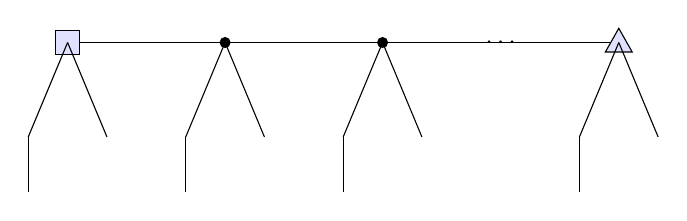
\begin{tikzpicture}[every node/.style={font=\small}]
		\draw (0,0) -- (7,0);
		\draw[fill=blue!12] (-0.15,-0.15) rectangle (0.15,0.15);
		\foreach \x in {2,4} \fill (\x,0) circle (2pt);
		\draw[fill=blue!12] (7,0.18) -- (6.83,-0.12) -- (7.17,-0.12) -- cycle;
		\node at (5.5,0) {$\cdots$};
		\foreach \x in {0,2,4,7} {
			\draw (\x,0) -- (\x-0.5,-1.2);
			\draw (\x,0) -- (\x+0.5,-1.2);
			\draw (\x-0.5,-1.2) -- (\x-0.5,-1.9);
		}
	\end{tikzpicture}
\end{center}

\begin{Definition}{ЭПФ последовательностей}{seq}
	ЭПФ непустых линейно упорядоченных наборов: $S(x)=\sum_{k\ge 1}k!\dfrac{x^k}{k!}=\dfrac{x}{1-x}$.
\end{Definition}

\begin{Statement}{Композиционная формула}{compose}
	$\widehat T(x)=S(T(x))=\sum_{d\ge 1}T(x)^d$.
\end{Statement}

\begin{proof}
	$T(x)^d$ — ЭПФ упорядоченных наборов из $d$ корневых деревьев: $[x^n]T(x)^d=\sum_{a_1+\dots+a_d=n}\frac{\widetilde t_{a_1}}{a_1!}\cdots\frac{\widetilde t_{a_d}}{a_d!}$. Сумма по $d\ge 1$ даёт $S(T(x))$; каждый набор отвечает дереву, у которого корни поддеревьев соединены в путь, а концы пути — две отмеченные вершины.
\end{proof}

\begin{Lemma}{Жуаль: дважды отмеченные деревья и отображения}{joyal}
	\[
	S(T(x))=\sum_{n\ge 1}n^n\frac{x^n}{n!},\qquad\text{т.е.}\qquad \widetilde{\widetilde t}_n=n^n.
	\]
\end{Lemma}

\begin{Remark}{Идея биекции}{}
	Дважды отмеченное («позвоночное») дерево на $[n]$ биективно соответствует произвольному отображению $[n]\to[n]$. Функциональный граф отображения — набор циклов, на которых висят корневые деревья; перестановка вершин хребта (циклы) заменяется линейным порядком (последовательностью $S$) и обратно. Всех отображений $[n]\to[n]$ ровно $n^n$, откуда ЭПФ $\sum_n n^n x^n/n!$.
\end{Remark}

\begin{proof}[Завершение доказательства формулы Кэли]
	Из леммы $\widetilde{\widetilde t}_n=n^n$, а по определению $\widetilde{\widetilde t}_n=n^2 t_n$. Значит, $n^2 t_n=n^n$, откуда $t_n=n^{n-2}$.
\end{proof}

\subsection{Связанный сюжет: парковочные функции и игра в фишки}

\begin{Definition}{Парковочная функция}{parking}
	Есть $n$ ячеек $0,\dots,n-1$ и $n$ машин. Машина $i$ едет к ячейке $a_i$ и паркуется в ней, если свободна, иначе — в ближайшую свободную впереди. Набор $(a_1,\dots,a_n)$, $a_i\in\{0,\dots,n-1\}$, — \emph{парковочная функция}, если все машины паркуются.
\end{Definition}

\begin{Statement}{Критерий парковки}{park-crit}
	Пусть $a_{(1)}\le\dots\le a_{(n)}$ — отсортированные предпочтения. Все паркуются $\iff a_{(i)}\le i-1$ для всех $i$.
\end{Statement}

\begin{proof}
	Если $a_{(i)}\ge i$ для некоторого $i$, то $n-i+1$ машин хотят ячейки $\ge i$, которых лишь $n-i$ — не хватит. Обратно, при $a_{(i)}\le i-1$ обработка в отсортированном порядке всегда ставит $i$-ю машину не дальше ячейки $i-1$.
\end{proof}

\begin{Example}{Малые значения}{small}
	$n=2$: $(0,0),(0,1),(1,0)$ — $3$ штуки. $n=3$: $1+3+3+3+6=16$. $n=4$: $1+12+36+12+64=125$. Последовательность $1,1,3,16,125=(n+1)^{n-1}$.
\end{Example}

\begin{Theorem}{Число парковочных функций}{parking-count}
	Число парковочных функций длины $n$ равно $(n+1)^{n-1}$.
\end{Theorem}

\begin{proof}[Идея]
	Это число остовных деревьев $K_{n+1}$: по формуле Кэли $(n+1)^{(n+1)-2}=(n+1)^{n-1}$. Парковочные функции ставятся в биекцию с остовными деревьями $K_{n+1}$ (равносильно — с рекуррентными конфигурациями игры в фишки на $K_{n+1}$).
\end{proof}

\subsubsection*{Игра в фишки на $K_{n+1}$}

Рассмотрим $K_{n+1}$ с выделенной вершиной-стоком; остальные — $1,\dots,n$.

\begin{Remark}{Редуцированный лапласиан}{laplacian}
	Пусть $L'_{K_{n+1}}$ — лапласиан без строки и столбца стока. По матричной теореме о деревьях $\det L'_{K_{n+1}}=\#\{\text{остовных деревьев }K_{n+1}\}=(n+1)^{n-1}$.
\end{Remark}

\begin{Definition}{Выстрел вершины}{firing}
	В вершине $i$ лежит $a_i$ фишек. \emph{Выстрел} (при $a_i\ge d_i$) уменьшает запас на степень $d_i$ и добавляет по фишке каждому соседу: $a_i\to a_i-d_i$, $a_j\to a_j+1$ ($j\sim i$).
\end{Definition}

\begin{Statement}{Рекуррентные конфигурации}{recurrent}
	Число стабильных (нередуцируемых выстрелами) конфигураций равно $\bigl|\mathbb Z^n/L'_{K_{n+1}}\mathbb Z^n\bigr|=|\det L'_{K_{n+1}}|=(n+1)^{n-1}$.
\end{Statement}

\begin{Remark}{Итог}{}
	Парковочные функции $\leftrightarrow$ рекуррентные конфигурации игры в фишки на $K_{n+1}$ $\leftrightarrow$ остовные деревья $K_{n+1}$; их число $\det L'_{K_{n+1}}=(n+1)^{n-1}$, что согласуется с формулой Кэли.
\end{Remark}
